


\chapter{Docking computazionale}
\textit{In questo capitolo vengono introdotte le nozioni, i concetti e le terminologie fondamentali che verranno utilizzati, in seguito, all'interno di questo elaborato.
In questo capitolo si vogliono fornire le basi, nell'ambito
del docking molecolare, propedeutiche ed
indispensabili per la comprensione dei capitoli successivi $\ldots$}

\vskip 1cm
\section{Docking molecolare} \label{docking_molecolare}
Sebbene sia un processo naturale che si verifica all'interno di una cellula, dal punto di vista computazionale il termine \textit{"docking molecolare"} si riferisce ad indagare come due o più strutture molecolari si adattano insieme.
In altre parole, il \textit{docking} è una tecnica di modellazione molecolare che viene utilizzata per prevedere come una proteina (enzima) interagisce con piccole molecole (ligandi) \cite{roy_chapter_2015}.

La capacità di una proteina di interagire con piccole molecole per formare un complesso supramolecolare gioca un ruolo importante nella dinamica della proteina, che può aumentare o inibire la sua funzione biologica \cite{roy_chapter_2015}.

Le interazioni intermolecolari tra proteina e ligando possono essere interazioni elettrostatiche, di van der Waals e idrofobiche, etc. Queste interazioni formano un complesso proteina-ligando che deve essere analizzato a livello atomico \cite{naqvi_advancements_nodate}.

La tecnica del docking molecolare, quindi, mira a identificare le possibili \textit{pose}\footnote{Binding pose, in inglese, indica la posizione, conformazione ed orientamento con cui il ligando può legarsi ad un recettore.} del ligando nel \textit{sito di binding}\footnote{Binding site, in inglese, indica la regione su una macromolecola come una proteina che si lega a un'altra molecola con specificità.} di una proteina ed a predire l'affinità tra il ligando e la proteina \cite{roy_chapter_2015}.

\begin{figure}[H]
    \centering
    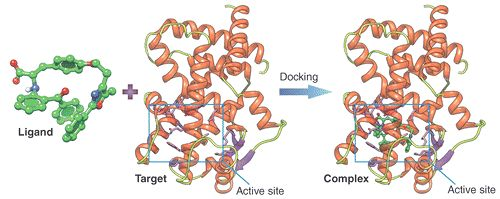
\includegraphics[scale=0.8]{images/chapter1/docking.jpg}
    \caption[Illustrazione grafica del complesso proteina-ligando.]{Illustrazione grafica del complesso proteina-ligando. Sulla sinistra il ligando, al centro la proteina (il riquadro mette in evidenza il sito attivo), a destra la conformazione proteina-ligando a seguito del docking. Fonte: \cite{liao_molecular_2013}}
    \label{fig:molecular_docking}
\end{figure}

In base ai tipi di ligando, il docking può essere classificato come
\begin{itemize}
    \item \textbf{Proteina-ligando}: rappresenta la casistica più semplice dello spettro di complessità e ci sono molti programmi disponibili che funzionano particolarmente bene nel predire le molecole che possono potenzialmente inibire le proteine. 
    A sua volta, il docking proteina-ligando può essere classificato nel modo seguente: 
    \begin{itemize}
        \item[◦] \textbf{Rigid-body docking}, in cui sia il recettore che il ligando sono trattati come rigidi; 
        \item[◦] \textbf{Flexible ligand docking}, in cui il recettore è tenuto rigido, ma il ligando è trattato come flessibile. E' il modello  utilizzato comunemente dagli algoritmi di docking;
        \item[◦] \textbf{Flexible docking}, in cui si considera sia la flessibilità del recettore che del ligando \cite{roy_chapter_2015}.
    \end{itemize}
    \item \textbf{Proteina-acido nucleico}: riguarda processi biologici essenziali, tra cui la replicazione del DNA, la trascrizione dell'RNA, etc. Tuttavia, la determinazione sperimentale della maggior parte delle strutture complesse proteina-acido nucleico con metodi ad alta risoluzione è un processo noioso e difficile.
    \item \textbf{Proteina-proteina}: è in genere molto più complesso. Il motivo è dato dal fatto che le proteine sono flessibili e il loro spazio conformazionale è piuttosto vasto.
\end{itemize}

E' importante sottolineare che le prestazioni del docking dipendono dall'algoritmo di ricerca. Inolte, al fine di evitare fonti di incomprensione od ambiguità, occorre fare una breve premessa sulla terminologia tecnica.


Distinguiamo tra energia di legame e affinità di legame.
L'affinità di legame è un termine usato per trovare l'efficienza del complesso ligando-recettore valutando le interazioni presenti nel complesso attraverso funzioni di scoring, campo di forza e metodi statistici.
L'energia libera di legame o \textit{binding energy} è la somma di tutte le interazioni intermolecolari presenti tra il ligando ed il recettore e può essere utilizzata come una stima di affinità di legame.

L'energia rilasciata a causa della formazione del legame, o meglio, dell'interazione del ligando e della proteina è definita sotto forma di "binding energy" o energia di legame. L'energia libera della reazione favorevole è negativa. Minore è l'energia di legame, migliore è il legame del ligando e della proteina, più il complesso sarà stabile.

\subsection{Breve storia del docking molecolare}
Il legame di una proteina ai ligandi ha una notevole rilevanza nel moderno processo di drug discovery\footnote{Con il termine \textit{drug discovery} s'intende il processo attraverso il quale vengono scoperti nuovi farmaci candidati.}, per tal motivo il docking molecolare è una tecnica ampiamente utilizzata dall'inizio degli anni '80.
Il docking molecolare è stato descritto per la prima volta nel 1982 dallo scienziato americano Tack Kuntz e da allora è diventato l'idea centrale nello \textit{structure-based virtual screening}.
In tempi moderni, la biologia strutturale si sta espandendo giorno dopo giorno, al punto che viene utilizzata da una serie di tecniche computazionali avanzate come l'\textit{high-throughput virtual screening} (vHTS) \cite{noauthor_chapter_nodate,naqvi_advancements_nodate}.
Tuttavia, esistono anche alcune limitazioni delle attuali tecniche di docking, tra cui la complessità, la flessibilità dei ligandi e delle proteine, ecc. \cite{naqvi_advancements_nodate}


\subsection{Passi elementari del docking}
Fondamentalmente, il docking è un processo in tre fasi indipendentemente dal software e dagli algoritmi di docking. 
Il primo passo è la \textbf{preparazione dei ligandi}. In questo processo, tutte le strutture duplicate devono essere rimosse e i parametri per i rispettivi ligandi devono essere impostati nella piattaforma software funzionante \cite{roy_chapter_2015}.

\begin{figure}[H]
    \centering
    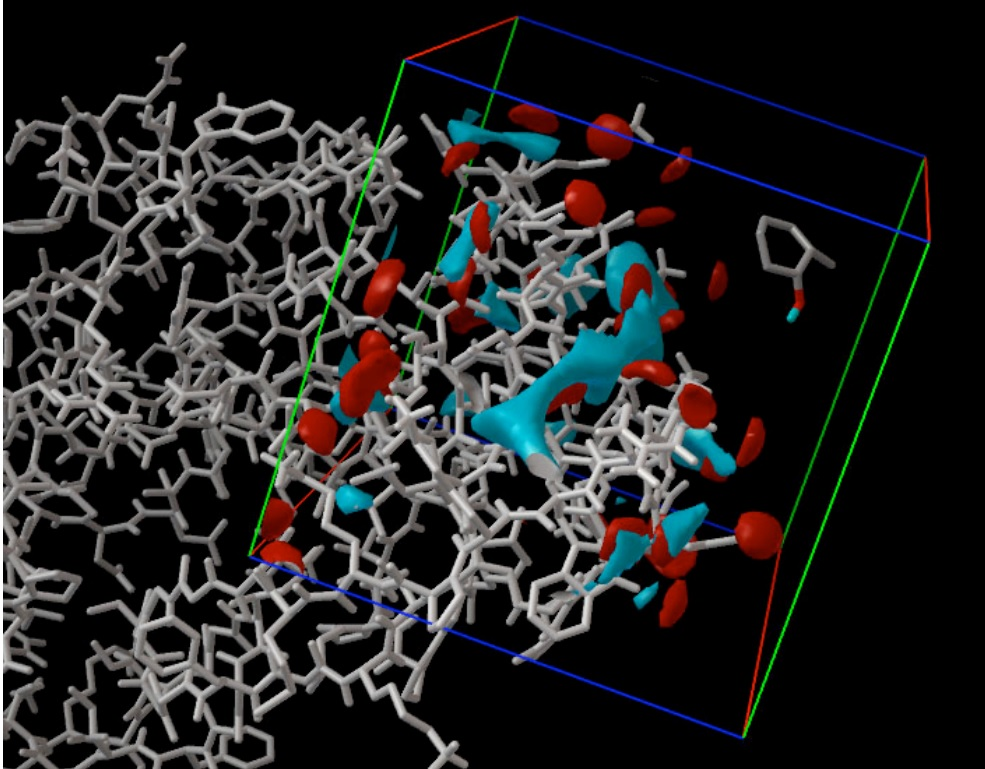
\includegraphics[scale=0.5]{images/chapter1/gridbox.jpg}
    \caption[Rappresentazione visiva di una gridbox in AutoDockTools]{Rappresentazione visiva di una gridbox all'interno di AutoDockTools. La gridbox è rappresentata da un cubo dai lati colorati di rosso, verde e blu. In grigio la struttura proteica, in azzurro è rappresentato il ligando ed in rosso le collisioni tra le strutture. Fonte: \cite{eberhardt_autodock_nodate}}
    \label{fig:gridbox}
\end{figure}

Il secondo passo è la \textbf{preparazione della proteina}: 
\begin{itemize}
    \item è necessario aggiungere atomi di idrogeno, seguito dalla rimozione delle molecole d'acqua tranne nel sito attivo;
    \item la proteina dovrebbe essere regolata correggendo eventuali errori gravi come residui incompleti vicino al sito attivo;
    \item le cariche e i tipi di atomi per qualsiasi atomo di metallo dovrebbero essere impostati correttamente, se necessario;
    \item se ci sono legami con ioni metallici, i legami dovrebbero essere cancellati, quindi aggiustando le cariche formali degli atomi che erano attaccati al metallo, così come il metallo stesso. 
\end{itemize}
La molecola proteica, così preparata, costituisce il recettore pronto per il docking \cite{roy_chapter_2015}.

Dopo aver verificato che la proteina e i ligandi siano nella forma corretta per il docking, in alcuni casi si passa alla \textbf{generazione della gridbox} per ogni recettore. La \textit{gridbox}\footnote{La posizione della gridbox definisce la regione della proteina in cui verrà eseguito il docking. Qualsiasi regione al di fuori della gridbox non verrà esplorata durante il docking.} è generalmente generata al baricentro del ligando legato al sito attivo del recettore. 
In altri casi, vengono identificate cavità o sacche attive della proteina in cui fissare il ligando \cite{roy_chapter_2015}.

A questo punto del processo, viene effettuato il \textbf{docking proteina-ligando}, che consiste nella ricerca accurata del corretto orientamento e della corretta conformazione di un ligando all'interno di una cavità della proteina e nella valutazione di tali pose attraverso l'applicazione della funzione di scoring, la quale restituisce una misura di energia della posa, indicata con il termine \textit{affinità} \cite{roy_chapter_2015}.

\begin{figure}[h]
    \centering
    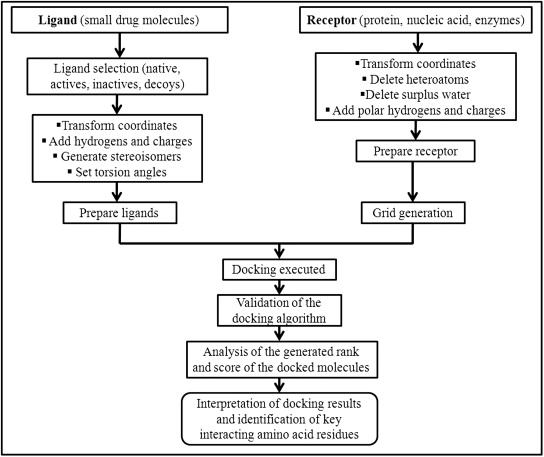
\includegraphics[scale=0.7]{images/chapter1/docking_steps.jpg}
    \caption[Schema riassuntivo dei passi del docking.]{Schema riassuntivo dei passi del docking. A sinistra la sequenza di passi per la preparazione dei ligandi, a destra la sequenza di passi per la preparazione delle proteine. Al centro è sintetizzato il processo di docking. Fonte: \cite{roy_chapter_2015}}
    \label{fig:docking_steps}
\end{figure}

Per ogni particolare posa viene contato il numero di interazioni intermolecolari favorevoli come legami idrogeno e contatti idrofobici. 
Al fine di riconoscere la posa energeticamente migliore, ogni posa viene valutata in base alla sua compatibilità con il target in termini di forma e proprietà e viene generato il punteggio corrispondente. Un buon punteggio per un dato ligando significa che è potenzialmente un buon legante \cite{roy_chapter_2015}.

Un determinato numero di pose del ligando viene salvato per ogni conformazione del ligando. Dopodichè viene effettuato il \textbf{ranking}, ovvero il processo di classificazione dei ligandi in cui le pose determinate e salvate per ciascuna conformazione del composto vengono ordinate in base ai rispettivi punteggi (cioè, le loro affinità previste).  Questo elenco ordinato viene quindi utilizzato per ulteriori sintesi e indagini biologiche solo per quei composti che si prevede siano più attivi \cite{roy_chapter_2015}.


\subsection{Requisiti essenziali per il docking} \label{requirements}
I requisiti essenziali per poter effettuare il docking molecolare riguardano la struttura molecolare del recettore così come le strutture di un insieme di ligandi di interesse.

La struttura del recettore può essere determinata mediante tecniche sperimentali come la cristallografia a raggi X o la spettrografia NMR. Tale struttura può essere facilmente scaricata dal \textit{Protein Data Bank}\footnote{Il \textit{Protein Data Bank} (PDB) è un archivio per dati di struttura in 3-D di proteine e acidi nucleici. Finora sono state depositate nel database PDB (http://www.rcsb.org) più di 140.000 strutture molecolari tridimensionali di diverse biomacromolecole tra cui molte proteine e complessi proteina-ligando \cite{naqvi_advancements_nodate}.} \cite{roy_chapter_2015}. 

La qualità della struttura del recettore gioca un ruolo cruciale nel successo del docking computazionale. In generale, maggiore è la risoluzione della struttura cristallina impiegata, migliori sono i risultati di docking osservati.

Un altro criterio importante per esaminare la qualità di una struttura recettoriale è il fattore Debye Waller (DWF)\footnote{Il fattore di Debye-Waller, noto anche come fattore B o fattore di temperatura, descrive la variazione dell'intensità di scattering (sia di raggi X, sia di neutroni) dovuta al moto termico degli atomi o al disordine del cristallo.}.

Al contrario, se la struttura cristallina a raggi X della proteina non è disponibile, si può optare per la predizione della struttura. In tal caso, le tecniche più comunemente applicate sono il \textit{“threading”} e l'\textit{“homology modeling”}. Nel caso del threading, viene effettuata una stima se una determinata sequenza di amminoacidi è compatibile con uno dei ligandi in un database.
D'altra parte, l'homology modeling si basa su una correlazione o omologia tra la sequenza della proteina-obiettivo ed almeno una struttura nota. \cite{roy_chapter_2015}

Le strutture dei ligandi di interesse sono ricavate da PubChem\footnote{PubChem è un database di molecole chimiche, gestito dal centro nazionale per l'Informazione biotecnologica statunitense (NCBI), parte della biblioteca nazionale di medicina (NLM) dell'istituto nazionale della sanità americano (NIH).} oppure dalle banche dati dedicate, messe a disposizione dalla Commissione Europea, come ad esempio l'EU Pesticides Database.


\section{Implementazione del docking molecolare} \label{implementazione_docking}
Come anticipato nella Sezione \ref{docking_molecolare}, il docking molecolare prevede una fase di campionamento dello spazio conformazionale del complesso proteina-ligando e una fase di valutazione della migliore conformazione trovata. 
Per poter esaminare lo spazio conformazionale, è necessario applicare un algoritmo di campionamento come ad esempio il campionamento di Monte Carlo. Le conformazioni campionate vengono valutate attraverso una funzione di scoring, che a sua volta applica un algoritmo di ottimizzazione come l'algoritmo di Broyden-Fletcher-Goldfarb-Shanno.
In questa sezione sono descritti il concetto di funzione di scoring e gli algoritmi che costituiscono il docking molecolare.

\subsection{Algoritmo di campionamento dello spazio conformazionale}
Lo spazio conformazionale del ligando viene esplorato utilizzando il \textbf{campionamento di Monte Carlo}; tendenzialmente le catene sono eseguite in parallelo utilizzando i threads della CPU. Il numero degli steps per le catene di Monte Carlo sono calcolati sulla base del numero degli atomi mobili e sul numero dei gradi di libertà all'interno del ligando. 

Ad ogni passo della catena di Monte Carlo, il ligando è modificato selezionando casualmente una delle seguenti operazioni: traslazione casuale, rotazione casuale dell'intera molecolare, o selezionando gli angoli di torsione del ligando in maniera casuale. 

Il processo di Monte Carlo prevede il ripristino casuale degli angoli di torsione con una probabilità maggiore rispetto alle altre mutazione. Dopo la mutazione, è effettuata una minimizzazione dell'energia approssimativa,  secondo una certa funzione di scoring, che può essere empirica (non-CNN) o CNN. 

\subsection{Funzioni di scoring}
Le funzioni di scoring forniscono una relazione dallo spazio conformazionale del ligando e del recettore all'insieme dei numeri reali in modo che le pose possano essere classificate. 
La forma e la parametrizzazione delle funzioni di scoring varia ampiamente tra le implementazioni \cite{mcnutt_gnina_2021}.

Tipicamente, le funzioni di scoring sono raggruppate in quattro categorie:
\begin{itemize}
    \item \textbf{basate sulla conoscenza}, derivate utilizzando statistiche per le frequenze di contatto interatomiche osservate, le distanze od entrambe, in un ampio database di strutture cristalline di complessi proteina-ligando. Le funzioni di scoring basate sulla conoscenza possono essere influenzate dalle caratteristiche presenti nei loro set di formazione sebbene i calcoli dei punteggi siano rapidi al momento del test. Richiedono un ampio database di strutture conosciute e possono essere difficili da interpretare quando si cerca di comprendere un punteggio \cite{mcnutt_gnina_2021, koes_lessons_2013}; 
    
    \item \textbf{basate sul campo di forza}, cercano di quantificare le effettive forze molecolari che esistono tra una proteina e una piccola molecola. Le interazioni di Van der Waals, le interazioni elettrostatiche e le interazioni di legame idrogeno sono componenti comuni delle funzioni di scoring basate sul campo di forza. Questi termini sono idealmente parametrizzati dai primi principi. Le funzioni di scoring del campo di forza sono spesso progettate per l'uso nelle simulazioni di dinamica molecolare. Tuttavia, l'accuratezza di tali funzioni basate sulla fisica è limitata dalla loro complessità e dalle ipotesi che poniamo sulle forze fondamentali che dettano le interazioni tra le molecole, sebbene la comprensione di queste forze sia in continuo aumento \cite{mcnutt_gnina_2021, koes_lessons_2013}; 
    
    \item \textbf{empiriche}, affrontano i limiti delle funzioni di punteggio basate sulla fisica utilizzando una combinazione di termini energetici selezionati manualmente. Invece di assegnare a ciascun termine energetico una ponderazione identica, i pesi di ciascun termine sono determinati tramite un adattamento ai dati sperimentali. Possono avere termini simili alle funzioni di scoring basate sul campo di forza e possono anche contenere termini più complessi ed euristici, come le interazioni idrofobiche. Come le funzioni di scoring basate sulla conoscenza, le prestazioni delle funzioni di scoring empiriche dipendono e migliorano con la quantità e la qualità dei dati di addestramento. Gran parte del software di docking utilizza funzioni di punteggio empirico, tra cui AutoDock Vina \cite{mcnutt_gnina_2021, koes_lessons_2013};
    \item \textbf{CNN}, prende in input una rappresentazione 3D di un complesso proteina-ligando ed apprende automaticamente le caratteristiche chiave delle interazioni correlate al legame. Le funzioni di scoring CNN possono essere addestrate ed ottimizzate per discriminare tra pose corrette e scorrette e leganti noti e non leganti \cite{mcnutt_gnina_2021}.
\end{itemize}

\subsection{Algoritmo di ottimizzazione} \label{bfgs}
Nell'implementazione della funzione di scoring Vina, utilizzata dai software che saranno presentati nel prossimo capitolo, viene utilizzato il metodo \textbf{Broyden-Fletcher-Goldfarb-Shanno} (BFGS) per l'ottimizzazione locale, che è un metodo quasi-Newton efficiente. 
BFGS è un metodo iterativo per risolvere problemi di ottimizzazione non lineare non vincolata e, come altri metodi di ottimizzazione quasi-Newton, utilizza non solo il valore della funzione di scoring ma anche il suo gradiente, ovvero le derivate della funzione di scoring rispetto ai suoi argomenti. Gli argomenti, nel nostro caso, sono la posizione e l'orientamento del ligando, così come i valori delle torsioni per i legami ruotabili attivi nel ligando e gli eventuali residui flessibili \cite{trott_autodock_2009}.

Sebbene la valutazione del gradiente oltre al valore della funzione di scoring stessa possa richiedere più tempo, il suo utilizzo può accelerare notevolmente l'ottimizzazione. Il numero di iterazioni in un'esecuzione è determinato in modo adattivo, in base all'apparente complessità del problema, e vengono eseguite più esecuzioni a partire da conformazioni casuali. Queste esecuzioni possono essere eseguite contemporaneamente, utilizzando il multithreading. Ciò consente di sfruttare il parallelismo hardware a memoria condivisa, come le ormai onnipresenti CPU multicore. L'algoritmo di ottimizzazione mantiene una serie di diversi minimi significativi trovati che vengono quindi combinati da esecuzioni separate e utilizzati durante la fase di perfezionamento della struttura e clustering \cite{trott_autodock_2009}.

L'analisi di clustering è il modo migliore per determinare se la simulazione ha ispezionato adeguatamente lo spazio conformazionale disponibile \cite{forli_computational_2016}. Questa consiste nell'eseguire più simulazioni di docking e confermare che la migliore conformazione viene trovata più volte.

\section{Virtual Screening}
Nella modellazione di farmaci basata sulla struttura, ottenere il modello più accurato ed efficiente di complesso ligando-recettore è un passaggio cruciale ed è un punto di partenza adatto per ulteriori valutazioni per testare nuovi composti o possibili farmaci candidati \cite{menchaca_past_2020}.
 
Il \textit{virtual screening} o il \textit{virtual high-throughput screening} (vHTS) è una potente tecnica computazionale utilizzata nel processo di scoperta di farmaci per identificare piccoli composti bioattivi, mediante la ricerca in alcune librerie chimiche, che possono legarsi efficacemente ad un particolare farmaco target, e che possono essere usati come riferimento o \textit{lead compounds}\footnote{Lead compounds, composti guida} \cite{naqvi_advancements_nodate}.

L'accuratezza di questa tecnica è notevolmente migliorata negli ultimi anni e ciò ha permesso di far ormai parte ad una serie di tecniche computazionali che consentono ai ricercatori di ridurre una vasta libreria di composti ad una dimensione più conveniente. Queste tecniche consentono la valutazione di ampie librerie di composti chimici rispetto ad un target biologico ma soprattutto uno screening rapido ed efficace \cite{naqvi_advancements_nodate}.

Gli approcci VS sono stati vigorosamente implementati dalle industrie farmaceutiche con l'intento di ottenere il maggior numero possibile di potenziali composti, con la speranza di una maggiore possibilità di trovare risultati dall'ampio pool disponibile di librerie chimiche. Molti esempi di successo sono stati dimostrati di recente nell'identificazione di lead compounds \cite{roy_chapter_2015}.

Tuttavia, l'approccio VS dipende fortemente dalla quantità e qualità dei dati disponibili e dalla capacità di predizione dell'algoritmo sottostante. Di conseguenza, non esiste una linea guida o un flusso di lavoro universale per queste tecniche, per cui il ricercatore deve applicare la sua conoscenza ed esperienza computazionale per trovare il farmaco candidato attivo tra grandi database di farmaci e librerie chimiche, applicando i migliori strumenti possibili secondo le sue esigenze \cite{roy_chapter_2015}.

Inoltre, poiché ogni target biologico è unico, non sembra esserci un metodo universale per eseguire questi studi.

\begin{figure}[H]
    \centering
    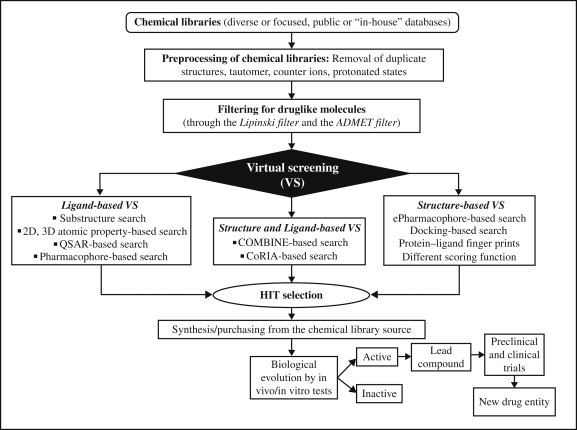
\includegraphics[scale=0.8]{images/chapter1/virtual_screening.jpg}
    \caption[Passi nell'applicazione del virtual screening.]{Passi nell'applicazione del virtual screening. A seguito di una fase di preprocessing, vengono illustrati differenti approcci di virtual screening ed infine vengono trattati possibili hit in vivo/in vitro per classificare il sito come attivo o inattivo. Fonte: \cite{roy_chapter_2015}}
    \label{fig:virtual_screening}
\end{figure}

Sebbene non si possano ignorare le restrizioni intrinseche del VS, rimane una delle migliori opzioni possibili per esplorare un ampio spazio chimico, in termini di efficacia dei costi e impegno di tempo e materiale necessario. 
Con lo sviluppo di nuove metodologie di docking, tecniche di screening basate su ligandi e sistemi di \textit{machine learning}, le tecniche VS sono in grado di fornire \textit{hit prediction rate} migliori e, senza dubbio, svolgeranno un ruolo di primo piano nella progettazione di farmaci nel prossimo futuro sia come approccio complementare all'HTS o come approccio autonomo \cite{roy_chapter_2015}.

\section{Applicazione del docking computazionale} 
Nell'ambito della valutazione dei rischi, il docking computazionale ha un ruolo molto importante poiché, attraverso la potenza di calcolo delle macchine moderne e la quantità di strutture molecolari tridimensionali ottenute e memorizzate in grandi database, è possibile evitare e limitare gli esperimenti \textit{in vitro}, a favore dell'analisi delle interazioni \textit{in silico} ed a sostegno delle nuove metodologie di approccio (NAM), riconosciute dall'Agenzia statunitense per la protezione dell'ambiente (US EPA) \cite{us_epa_alternative_2017, scitovation_what_2021}.

La nascita del docking computazionale ha dato vita ad analisi di valutazione dei rischi condotte attraverso approcci computazionali efficaci, permettendo quindi di verificare e spiegare l'esistenza di una correlazione tra la tossicità di particolari pesticidi e la perdita di colonie di api mellifere, evitando il ricorso a tecniche di analisi \textit{in vitro}.
\subsection{Correlazione tra pesticidi ed api} \label{Apis mellifera}
Un esempio di applicazione del docking computazionale è sicuramente la valutazione dei rischi delle api mellifere esposte ai pesticidi comunemente utilizzati nell'agricoltura moderna.
La tematica è stata centrale nel lavoro di tirocinio interno presso il Consiglio Nazionale delle Ricerche (CNR), seguiti dal Prof. Angelo Ciaramella e dal Dott. Ferdinando Febbraio, svolto assieme al collega Alfredo Mungari, anch'egli laureando in Informatica Parthenope. 

L'attività svolta è partita da un'analisi di valutazione dei rischi,
condotta dal Dott. Ferdinando Febbraio e dalla Dott.ssa Mónica del Águila, biologa ambientale specializzata in Ecotossicologia, riguardo una correlazione tra pesticidi e le proteine da api mellifere con struttura 3D nota. Questo studio ha portato alla realizzazione di un software di supporto per l'automatizzazione di processi inerenti al docking computazionale.

\subsubsection{L'importanza degli impollinatori}
L'impollinazione delle api offre un'ampia varietà di benefici all'umanità, contribuendo alla trasformazione degli alimenti, alle materie prime, ai medicinali, alle fibre, ai valori sociali e culturali e al mantenimento della biodiversità e della protezione ambientale.

In botanica, l’impollinazione è definita come quel processo che consiste nel trasporto dei pollini dalla parte maschile e quella femminile dell’apparato riproduttivo delle piante, all'interno dello stesso fiore (self-pollination) o tra le piante (cross-pollination). 

Attualmente, il 5-8\% di tutta la produzione agricola globale andrebbe persa senza i servizi di impollinazione forniti dalle api, rendendo necessari cambiamenti nella dieta umana e l'espansione dei terreni agricoli per risolvere le carenze nella produzione agricola \cite{khalifa_overview_2021}. 

La riduzione della popolazione delle api ha destato una forte preoccupazione negli ultimi anni poiché rappresenta tutt'oggi un problema di globale importanza.
\cite{di_prisco_neonicotinoid_2013,li_neonicotinoid_2015}.

La perdita di impollinatori, i quali hanno un ruolo fondamentale nella produzione agricola mondiale, impatta indirettamente anche sul mercato globale, specie per i paesi che basano una buona parte della propria economia sui prodotti in cui interviene, in qualche maniera, l'impollinazione da insetti, ed in particolare delle api. In relazione ai loro orientamenti agricoli, alcune regioni sono apparse più vulnerabili come il Medio Oriente asiatico, l'Asia centrale, l'Asia orientale ed i paesi non appartenenti all'Unione Europea, principalmente importatori \cite{gallai_economic_2009}. Tuttavia, questo fenomeno colpisce quasi tutte le regioni del pianeta: questo ne motiva l'importanza e la drammaticità.

L'esposizione delle api a numerosi fattori di stress e l'impatto degli agenti patogeni, enfatizzato dall'esposizione a particolari pesticidi, ad esempio i neonicotinoidi\footnote{I neonicotinoidi sono insetticidi sistemici che vengono trasferiti nel polline e nel nettare di molte colture impollinate, è uno dei principali cofattori associati alla perdita di api.}, spiegano il collasso delle colonie, spesso associate ad alti livelli di infezione. 

I neonicotinoidi furono registrati per la prima volta agli anni '90 e nel 2010 rappresentarono un terzo del mercato globale degli insetticidi. La scarsa regolamentazione vigente fu la causa della loro diffusione, la quale fallì nel riconoscere i potenziali effetti ecologici ed ambientali del loro utilizzo \cite{sgolastra_bees_2020}. 

\subsubsection{CCD: Colony Collapse Disorder}

L'esposizione a prodotti chimici per l'agricoltura come fungicidi, insetticidi e pesticidi, causa contaminazione, tossicità e diminuzione della qualità e quantità dei nutrienti nel polline e nel nettare, portando a una cattiva salute delle colonie e quindi minacciando la sopravvivenza delle api (CCD\footnote{Il \textit{disturbo da collasso della colonia} (CCD) è un fenomeno per cui si verificano perdite rapide e inspiegabili di api da lavoro adulte in colonie di api gestite (ad esempio, colonie di api mellifere negli Stati Uniti), con il risultato che rimangono solo la regina e poche api che allattano.}, Colony Collapse Disorder).\cite{khalifa_overview_2021}.

\begin{figure}[H]
    \centering
    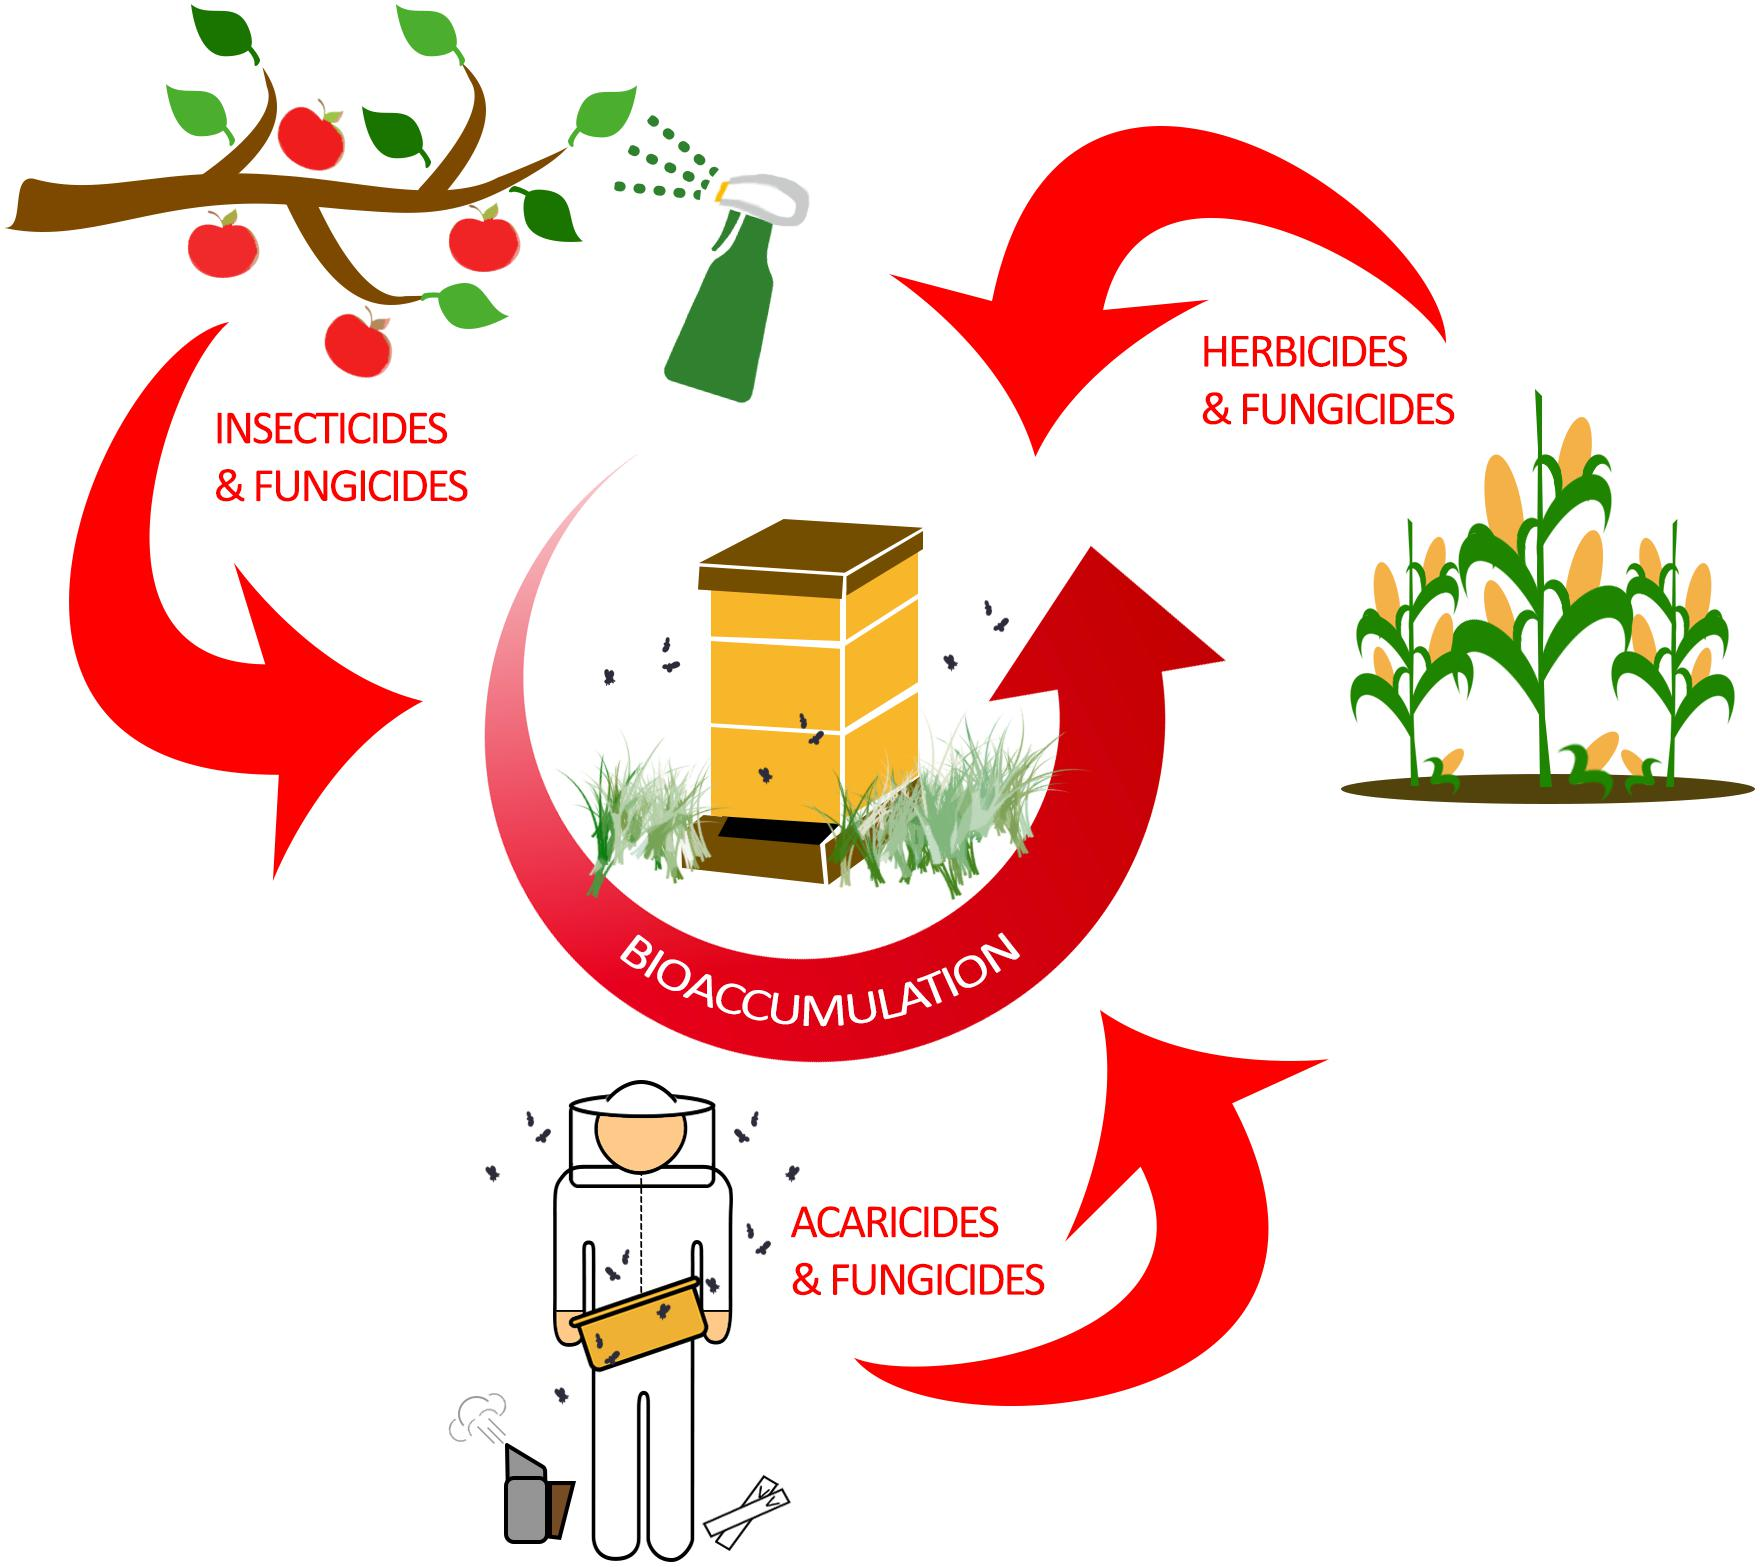
\includegraphics{images/chapter1/bioaccumulation.jpg}
    \caption[Bioaccumulo di pesticidi in una colonia di api mellifere.]{Bioaccumulo di pesticidi in una colonia di api mellifere. Le api mellifere sono esposte a un'ampia varietà di pesticidi attraverso pratiche agricole e l'apicoltura moderna. Mentre le api mellifere si nutrono di nettare e polline, sono accidentalmente esposte ai pesticidi che si accumulano nell'alveare trasferendo fisicamente le fonti di cibo contaminate alle api non esposte. Tuttavia, le api mellifere possono anche essere intenzionalmente esposte ad acaricidi e fungicidi dagli apicoltori nel tentativo di controllare il carico di acari e le malattie fungine nell'alveare. Fonte: \cite{chmiel_understanding_2020}}
    \label{fig:bioaccumulation}
\end{figure}

Poiché la tossicità è il principale fattore di rischio, le combinazioni sinergiche di fungicidi con particolari pesticidi sono fonte di grande preoccupazione poiché tale tossicità, già intrinsecamente elevata nei singoli composti, viene potenziata spaventosamente quando combinati insieme. 

Per questo motivo, l'esposizione ai pesticidi ad alte dosi è un fattore causale notevole coinvolto nel calo della popolazione delle api mellifere; tuttavia, l'esposizione ai pesticidi subletali presenta minacce non visibili per le api mellifere, portando a neurotossicità, immunodeficienza, cambiamenti comportamentali e disturbi cronici, oltre ad inficiare negativamente sulla riproduzione \cite{chmiel_understanding_2020}. 
